\documentclass[11pt]{article}

% NeurIPS-style standalone formatting, compatible with Overleaf/pdflatex.
\usepackage[margin=1in]{geometry}
\usepackage{times}
\usepackage{microtype}
\usepackage{amsmath,amssymb,amsthm,mathtools}
\usepackage{booktabs}
\usepackage{array}
\usepackage{enumitem}
\usepackage{xcolor}
\usepackage{hyperref}
\usepackage{tikz}
\usepackage{pgfplots}
\usepackage{caption}
\usepackage{subcaption}
\usepackage{fancyhdr}
\usepackage{titlesec}
\usetikzlibrary{arrows.meta,positioning,calc,fit,shapes,backgrounds,decorations.pathmorphing}
\pgfplotsset{compat=1.18}

\definecolor{deepblue}{RGB}{20,60,120}
\definecolor{softblue}{RGB}{225,238,255}
\definecolor{softgreen}{RGB}{226,246,232}
\definecolor{softred}{RGB}{255,230,230}
\definecolor{softgold}{RGB}{255,246,215}
\definecolor{darkgreen}{RGB}{35,120,60}
\definecolor{darkred}{RGB}{170,45,45}
\definecolor{darkgold}{RGB}{150,110,20}

\hypersetup{colorlinks=true, linkcolor=deepblue, citecolor=deepblue, urlcolor=deepblue}
\setlist[itemize]{leftmargin=1.3em, itemsep=0.18em, topsep=0.25em}
\setlist[enumerate]{leftmargin=1.5em, itemsep=0.18em, topsep=0.25em}
\titlespacing*{\section}{0pt}{1.4em}{0.6em}
\titlespacing*{\subsection}{0pt}{0.9em}{0.35em}
\titlespacing*{\subsubsection}{0pt}{0.7em}{0.25em}
\captionsetup{font=small, labelfont=bf}

\setlength{\headheight}{14pt}
\pagestyle{fancy}
\fancyhf{}
\lhead{ATS/AANA Camera-Ready Draft}
\rhead{\thepage}
\renewcommand{\headrulewidth}{0.4pt}

\newtheorem{definition}{Definition}
\newtheorem{theorem}{Theorem}
\newtheorem{proposition}{Proposition}
\newtheorem{corollary}{Corollary}
\newtheorem{assumption}{Assumption}
\newtheorem{remark}{Remark}

\newcommand{\KP}{K_P}
\newcommand{\KB}{K_B}
\newcommand{\KC}{K_C}
\newcommand{\Xstar}{X^*}
\newcommand{\Aglobal}{A_{\mathrm{global}}}
\newcommand{\Dglobal}{D_{\mathrm{global}}}
\newcommand{\Cglobal}{C_{\mathrm{global}}}
\newcommand{\eps}{\epsilon}
\newcommand{\gam}{\gamma}
\newcommand{\Rcal}{\mathcal{R}}
\newcommand{\Fcal}{\mathcal{F}}
\newcommand{\Scal}{\mathcal{S}}
\newcommand{\Mcal}{\mathcal{M}}

\title{\vspace{-1.5em}\textbf{Alignment-Aware Neural Architectures and Mechanistic Interoperability}\\
\large A Dynamical Theory of Constraint-Coherent Systems Under Scaling}

\author{Armando Sori\\
Independent Researcher\\
\texttt{research@simulateai.io}}
\date{May 2026}

\begin{document}
\maketitle
\thispagestyle{empty}

\begin{abstract}
Modern AI systems, agent networks, institutions, and digital platforms increasingly optimize internal objectives while drifting away from the real constraints that determine whether their outputs remain usable, safe, or socially viable. This paper develops a unified, camera-ready theory of Alignment-Aware Neural Architectures (AANA) and mechanistic interoperability (MI) as a special case of alignment dynamics in layered systems. We model reality as a layered constraint structure composed of physical or factual constraints, biological or human-impact constraints, constructed or task-level constraints, and feedback constraints. Alignment is defined as the probability mass of a system trajectory distribution inside a viable region of state space. Misalignment arises when optimization pressure acts through incomplete representations, misclassified constraints, weak feedback, irreversible loss, and inadequate correction capacity. 

The paper makes six contributions. First, it formalizes the ATS/AANA ontology of layered constraints. Second, it states alignment dynamics as a balance equation linking divergence pressure and correction capacity. Third, it derives the Alignment Incompleteness Law, Alignment Scaling Law, Correction Scaling Law, and Viable Design Space Theorem. Fourth, it specifies AANA as a systems architecture: generator, verifier stack, grounding module, correction policy, and alignment gate. Fifth, it formalizes mechanistic interoperability as network-level alignment coupling and proves that uncorrected interoperability can amplify global misalignment even when individual agents are locally stable. Sixth, it provides native TikZ figures and a NeurIPS-style submission checklist in a standalone Overleaf-compatible project. The central implication is conservative but operational: alignment is not a static property achieved through objective specification or verification alone. It is a dynamically maintained condition that requires correction capacity to scale at least as fast as pressure-amplified misclassification under incomplete feedback.
\end{abstract}

\section{Introduction}

Large-scale neural systems and multi-agent infrastructures are increasingly deployed as components in larger systems rather than as isolated models. Language models call tools, agents exchange outputs, platforms optimize engagement, institutions route decisions through automated pipelines, and markets synchronize through shared signals. These systems often exhibit the same structural failure pattern: internal performance improves while contact with underlying constraints degrades. A model becomes more fluent while hallucinating; a platform becomes more efficient at maximizing engagement while worsening user cognition; an institution improves internal scorecards while losing legitimacy; an interoperable agent network coordinates faster while propagating hidden errors.

This paper treats these failures as manifestations of a common dynamical structure: optimization under incomplete constraint representation. Systems do not act on reality directly. They act through internal models, proxy objectives, limited feedback, and finite verification procedures. When those representations omit or misclassify constraints, scaling coordination can amplify errors faster than local correction can absorb them. The result is not merely isolated model failure, but coordinated misalignment.

The proposed response is Alignment-Aware Neural Architectures (AANA). AANA adds explicit correction infrastructure around a base generator: verifier stack, grounding module, correction policy, and final alignment gate. The architecture does not guarantee perfect alignment. Instead, it makes a weaker and more defensible claim: systems should be designed to remain correctable under pressure. This reframes alignment as a control problem rather than a one-time specification problem.

\subsection{Core claim}

The core claim can be summarized as follows:
\begin{quote}
A system remains aligned under scaling only if correction capacity scales at least as fast as pressure-amplified misclassification under incomplete feedback.
\end{quote}
A compact version is
\begin{equation}
\frac{dA}{dt}= -\pi\eps(1-\gam)-\Lambda+C-\Phi,
\label{eq:alignment-dynamics}
\end{equation}
where $A$ is alignment, $\pi$ is optimization pressure, $\eps$ is misclassification error, $\gam$ is feedback fidelity, $\Lambda$ is irreversible loss, $C$ is correction capacity, and $\Phi$ is viable-region drift. Equation~\ref{eq:alignment-dynamics} is a coarse systems model, not a universal physical law. Its value is that it exposes the levers that any scalable alignment architecture must address.

\subsection{Contributions}

This paper contributes:
\begin{enumerate}
    \item a layered constraint ontology for AI and non-AI systems;
    \item a dynamical model of alignment as probability mass inside a viable region;
    \item named theoretical results: incompleteness, scaling, correction, viable design, and interoperability instability;
    \item a concrete AANA architecture for verifier-grounded correction;
    \item a formal treatment of mechanistic interoperability as alignment coupling across agent networks;
    \item native TikZ/PGFPlots figures and a NeurIPS-style checklist for submission readiness.
\end{enumerate}

\section{Related Work and Positioning}

\paragraph{Goodhart effects and proxy optimization.} Goodhart-style failures arise when optimized measures lose contact with the realities they were intended to represent. In machine learning, this appears as benchmark overfitting, reward hacking, and overoptimization of learned reward models. In institutions, it appears as metric compliance without mission fulfillment. This paper embeds those failures inside a layered constraint ontology: proxy failure is not only a metric problem, but a representation problem.

\paragraph{AI alignment and reward misspecification.} AI alignment research has long studied reward misspecification, distribution shift, truthfulness, calibration, tool misuse, and unsafe over-compliance. AANA is compatible with these concerns, but frames them architecturally: systems must be built with explicit mechanisms for detecting when outputs leave the feasible region and for correcting before propagation.

\paragraph{Control theory and verification.} Control theory emphasizes stability under feedback and disturbance. Formal verification certifies properties relative to a specification. AANA borrows from both traditions while acknowledging that finite verification is incomplete under partial observability. Verification alone cannot guarantee long-run alignment; it must be embedded in a persistent loop of grounding, scoring, correction, and monitoring.

\paragraph{Mechanistic interoperability.} Interoperability work often focuses on shared protocols, schemas, APIs, and representations. These are necessary for coordination, but not sufficient for alignment. A network can be syntactically interoperable while semantically and constraint-wise misaligned. This paper formalizes that gap.

\section{Layered Constraint Ontology}

\begin{definition}[Layered constraint structure]
Let a system operate over state or output space $X$. A layered constraint structure is
\begin{equation}
\Rcal=(\KP,\KB,\KC),
\end{equation}
where $\KP$ denotes physical, factual, material, or feasibility constraints; $\KB$ denotes biological, human-impact, cognitive, or social-viability constraints; and $\KC$ denotes constructed, institutional, policy, task-level, or metric constraints.
\end{definition}

In an AI system, $\KP$ includes factual truth, numerical validity, physical feasibility, and evidence support. $\KB$ includes safety, human impact, cognitive load, manipulation risk, uncertainty calibration, and harmful over-compliance. $\KC$ includes formatting, instructions, tool schemas, role constraints, benchmarks, and policy rules. The labels are engineering abstractions, not rigid metaphysical categories.

\begin{definition}[Viable region]
Let $\Xstar(\omega,\tau,\alpha)\subseteq X$ denote the viable region, parameterized by reference population $\omega$, time horizon $\tau$, and aggregation rule $\alpha$. A simplified constraint-intersection form is
\begin{equation}
\Xstar(t)=\KP(t)\cap\KB(t)\cap\KC(t).
\end{equation}
\end{definition}

\begin{definition}[Alignment]
Let $P_S(x,t)$ be the trajectory distribution induced by system $S$ over $X$, with density $p_S(x,t)$. Alignment is
\begin{equation}
A(S,t)=\int_{\Xstar(t)}p_S(x,t)\,dx.
\end{equation}
Misalignment is $M(S,t)=1-A(S,t)$.
\end{definition}

This definition makes alignment a trajectory-level property rather than a static certificate. A system may satisfy an objective locally while reducing its long-run probability mass inside the viable region.

\begin{figure}[t]
\centering
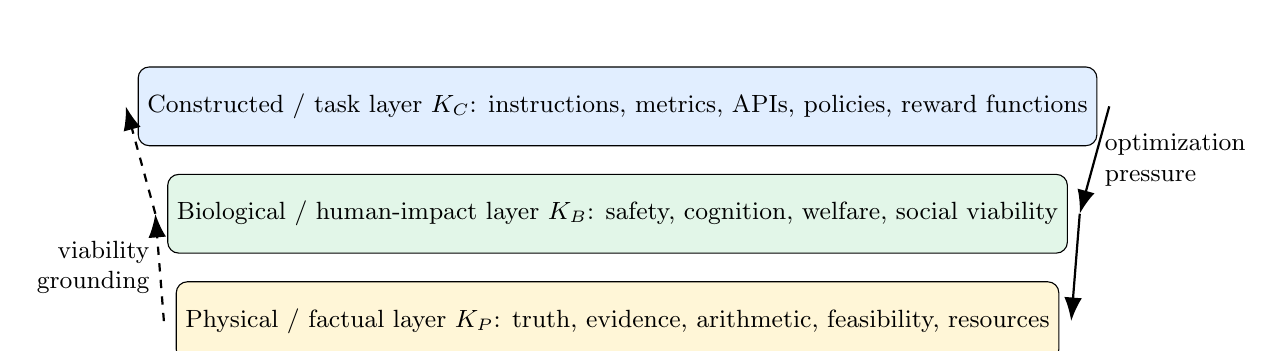
\begin{tikzpicture}[node distance=0.35cm, every node/.style={font=\small}]
\node[draw, rounded corners, fill=softblue, minimum width=10.5cm, minimum height=1.0cm] (c) {Constructed / task layer $K_C$: instructions, metrics, APIs, policies, reward functions};
\node[draw, rounded corners, fill=softgreen, minimum width=10.5cm, minimum height=1.0cm, below=of c] (b) {Biological / human-impact layer $K_B$: safety, cognition, welfare, social viability};
\node[draw, rounded corners, fill=softgold, minimum width=10.5cm, minimum height=1.0cm, below=of b] (p) {Physical / factual layer $K_P$: truth, evidence, arithmetic, feasibility, resources};
\draw[-{Latex[length=3mm]}, thick] ($(c.east)+(0.15,0)$) -- node[right, align=left]{optimization\\pressure} ($(b.east)+(0.15,0)$);
\draw[-{Latex[length=3mm]}, thick] ($(b.east)+(0.15,0)$) -- ($(p.east)+(0.15,0)$);
\draw[-{Latex[length=3mm]}, thick, dashed] ($(p.west)+(-0.15,0)$) -- node[left, align=right]{viability\\grounding} ($(b.west)+(-0.15,0)$);
\draw[-{Latex[length=3mm]}, thick, dashed] ($(b.west)+(-0.15,0)$) -- ($(c.west)+(-0.15,0)$);
\end{tikzpicture}
\caption{Layered constraint ontology. Constructed-layer success is often easiest to observe, but long-run viability is grounded by lower-layer factual, physical, biological, and human-impact constraints.}
\label{fig:layered-ontology}
\end{figure}

\subsection{Misclassification}

\begin{definition}[Representation map]
A finite system observes the world through a representation map
\begin{equation}
\phi:X\rightarrow M,
\end{equation}
where $M$ is an internal model space.
\end{definition}

\begin{definition}[Misclassification error]
Let $k$ denote a relevant constraint and let $\phi^*(k)$ denote its correct classification. A constraint is misclassified when $\phi(k)\ne\phi^*(k)$. The system-level misclassification rate is
\begin{equation}
\eps=\Pr\big(\phi(k)\ne\phi^*(k)\big).
\end{equation}
\end{definition}

Misclassification is not random noise. It is often incentivized. Treating factual uncertainty as answerable improves directness. Treating a safety constraint as a style preference permits over-compliance. Treating a hidden assumption as true allows fluency. These local gains can increase visible task performance while degrading alignment.

\section{Alignment Dynamics}

Let $\pi\ge 0$ denote optimization pressure, $\gam\in[0,1]$ feedback fidelity, $C\ge 0$ correction capacity, $\Lambda\ge 0$ irreversible loss, and $\Phi\ge 0$ viable-region drift. Alignment evolves according to Equation~\ref{eq:alignment-dynamics}. Define total divergence pressure as
\begin{equation}
D(S,t)=\pi\eps(1-\gam)+\Lambda+\Phi.
\end{equation}
Then
\begin{equation}
\frac{dA}{dt}=C-D.
\end{equation}
The critical stability condition is therefore
\begin{equation}
C\ge D.
\label{eq:critical-boundary}
\end{equation}

\begin{figure}[t]
\centering
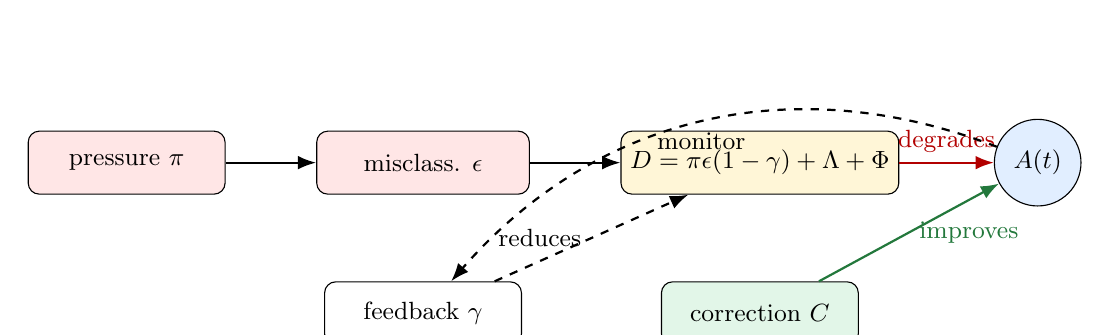
\begin{tikzpicture}[node distance=1.15cm, every node/.style={font=\small}]
\node[draw, rounded corners, fill=softred, minimum width=2.5cm, minimum height=0.8cm] (pi) {pressure $\pi$};
\node[draw, rounded corners, fill=softred, right=of pi, minimum width=2.7cm, minimum height=0.8cm] (eps) {misclass. $\epsilon$};
\node[draw, rounded corners, fill=softgold, right=of eps, minimum width=2.4cm, minimum height=0.8cm] (div) {$D=\pi\epsilon(1-\gamma)+\Lambda+\Phi$};
\node[draw, rounded corners, fill=softgreen, below=1.1cm of div, minimum width=2.5cm, minimum height=0.8cm] (corr) {correction $C$};
\node[draw, circle, fill=softblue, right=1.2cm of div, minimum size=1.1cm] (A) {$A(t)$};
\node[draw, rounded corners, fill=white, below=1.1cm of eps, minimum width=2.5cm, minimum height=0.8cm] (gamma) {feedback $\gamma$};
\draw[-{Latex}, thick] (pi) -- (eps);
\draw[-{Latex}, thick] (eps) -- (div);
\draw[-{Latex}, thick, red!70!black] (div) -- node[above]{degrades} (A);
\draw[-{Latex}, thick, darkgreen] (corr) -- node[right]{improves} (A);
\draw[-{Latex}, thick, dashed] (gamma) -- node[left]{reduces} (div);
\draw[-{Latex}, thick, dashed] (A) to[bend right=35] node[below]{monitor} (gamma);
\end{tikzpicture}
\caption{Alignment dynamics as a correction problem. Optimization pressure amplifies misclassification under incomplete feedback. Alignment is maintained when correction capacity exceeds divergence pressure.}
\label{fig:alignment-loop}
\end{figure}

\section{Main Theoretical Results}

\begin{theorem}[Alignment Incompleteness Law]
Let $\phi:X\to M$ be a finite representation of a higher-dimensional or partially observable state space $X$. If alignment depends on distinctions in $X$ not preserved by $\phi$, then there exists a nonzero lower bound on alignment-estimation error for any verifier operating only on $M$.
\end{theorem}
\begin{proof}[Proof sketch]
Since $M$ is finite or lower-resolution relative to $X$, there exist distinct states $x_1,x_2\in X$ such that $\phi(x_1)=\phi(x_2)$ while $x_1$ and $x_2$ differ in alignment-relevant membership relative to $\Xstar$. A verifier that observes only $\phi(x)$ cannot distinguish these states. Therefore its alignment estimate must assign the same value to states with different true viability status, inducing irreducible error. Additional data can reduce the empirical frequency of the error, but cannot eliminate the structural loss unless the representation itself preserves the missing distinction.
\end{proof}

\begin{theorem}[Alignment Scaling Law]
If $\eps>0$ and $\gam<1$, then increasing optimization pressure $\pi$ increases divergence pressure $D=\pi\eps(1-\gam)+\Lambda+\Phi$ unless $\eps$, $\gam$, $\Lambda$, or $\Phi$ improve sufficiently.
\end{theorem}
\begin{proof}
For fixed $\eps>0$ and $\gam<1$, $\partial D/\partial \pi=\eps(1-\gam)>0$. Thus increasing $\pi$ increases $D$ unless other terms change in compensation.
\end{proof}

\begin{theorem}[Correction Scaling Law]
A system maintains non-decreasing alignment at the margin only if correction capacity satisfies $C\ge D$.
\end{theorem}
\begin{proof}
From Equation~\ref{eq:alignment-dynamics}, $dA/dt=C-D$. Non-decreasing alignment requires $dA/dt\ge 0$, hence $C\ge D$.
\end{proof}

\begin{theorem}[Viable Design Space Theorem]
Let $X$ denote a representable design space and $\Xstar\subseteq X$ the viable region. Under alignment dynamics, a design is sustainably realizable only if its induced trajectory remains in $\Xstar$ and satisfies $C\ge D$. If optimization pressure increases while correction capacity does not scale with $D$, the stable subset of viable designs contracts.
\end{theorem}
\begin{proof}[Proof sketch]
A design whose trajectory exits $\Xstar$ violates at least one lower-layer or task-level constraint. Since $dA/dt=C-D$, when $C<D$ alignment decreases. Sustained negative alignment drift eventually reduces the probability mass inside the stable subset of $\Xstar$. Increasing $\pi$ increases $D$ by the Alignment Scaling Law. Therefore, absent compensating correction, the set of trajectories satisfying stability contracts.
\end{proof}

\begin{figure}[t]
\centering
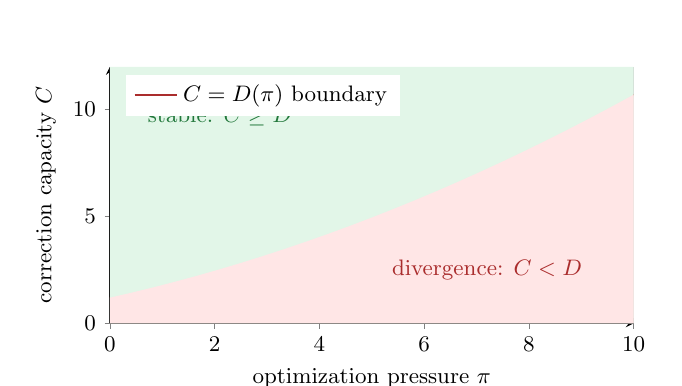
\begin{tikzpicture}[scale=0.9, every node/.style={font=\small}]
\begin{axis}[
width=0.74\textwidth,
height=5.2cm,
xlabel={optimization pressure $\pi$},
ylabel={correction capacity $C$},
xmin=0,xmax=10,ymin=0,ymax=12,
axis lines=left,
grid=both,
legend style={at={(0.03,0.97)},anchor=north west,draw=none,fill=white},
]
\addplot[domain=0:10, samples=100, thick, darkred]{1.2 + 0.55*x + 0.04*x^2};
\addlegendentry{$C=D(\pi)$ boundary}
\addplot[fill=softgreen, draw=none, domain=0:10] {12} \closedcycle;
\addplot[fill=softred, draw=none, domain=0:10] {1.2 + 0.55*x + 0.04*x^2} \closedcycle;
\node[darkgreen] at (axis cs:2.1,9.7) {stable: $C\ge D$};
\node[darkred] at (axis cs:7.2,2.5) {divergence: $C<D$};
\end{axis}
\end{tikzpicture}
\caption{Viable design stability boundary. Increasing pressure raises divergence pressure. Stable design requires correction capacity to scale with the boundary.}
\label{fig:phase-boundary}
\end{figure}

\section{Alignment-Aware Neural Architectures}

\begin{definition}[AANA system]
An Alignment-Aware Neural Architecture is a tuple
\begin{equation}
S=(f_\theta,E_\varphi,R,\Pi_\psi,G),
\end{equation}
where $f_\theta$ is a base generator, $E_\varphi$ a verifier stack, $R$ a retrieval or grounding module, $\Pi_\psi$ a correction policy, and $G$ an alignment gate.
\end{definition}

The inference loop is
\begin{align}
y_0 &\leftarrow f_\theta(x),\\
s_t &\leftarrow E_\varphi(x,y_t,e_t,m_t),\\
e_t &\leftarrow R(x,y_t),\\
a_t &\leftarrow \Pi_\psi(x,y_t,s_t,e_t,m_t),\\
y_{t+1}&\leftarrow T_{a_t}(x,y_t,s_t,e_t).
\end{align}
The action space is
\begin{equation}
\mathcal{A}=\{\mathrm{accept},\mathrm{revise},\mathrm{retrieve},\mathrm{ask},\mathrm{refuse},\mathrm{defer}\}.
\end{equation}

\begin{figure}[t]
\centering
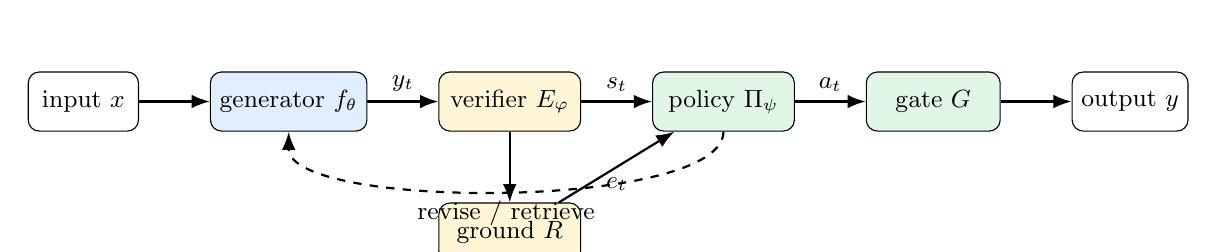
\begin{tikzpicture}[node distance=0.9cm, every node/.style={font=\small}]
\node[draw, rounded corners, fill=white, minimum width=1.4cm, minimum height=0.75cm] (input) {input $x$};
\node[draw, rounded corners, fill=softblue, right=of input, minimum width=1.8cm, minimum height=0.75cm] (gen) {generator $f_\theta$};
\node[draw, rounded corners, fill=softgold, right=of gen, minimum width=1.8cm, minimum height=0.75cm] (ver) {verifier $E_\varphi$};
\node[draw, rounded corners, fill=softgold, below=of ver, minimum width=1.8cm, minimum height=0.75cm] (ret) {ground $R$};
\node[draw, rounded corners, fill=softgreen, right=of ver, minimum width=1.8cm, minimum height=0.75cm] (pol) {policy $\Pi_\psi$};
\node[draw, rounded corners, fill=softgreen, right=of pol, minimum width=1.7cm, minimum height=0.75cm] (gate) {gate $G$};
\node[draw, rounded corners, fill=white, right=of gate, minimum width=1.4cm, minimum height=0.75cm] (out) {output $y$};
\draw[-{Latex}, thick] (input) -- (gen);
\draw[-{Latex}, thick] (gen) -- node[above] {$y_t$} (ver);
\draw[-{Latex}, thick] (ver) -- node[above] {$s_t$} (pol);
\draw[-{Latex}, thick] (ret) -- node[below] {$e_t$} (pol);
\draw[-{Latex}, thick] (pol) -- node[above] {$a_t$} (gate);
\draw[-{Latex}, thick] (gate) -- (out);
\draw[-{Latex}, thick] (ver) -- (ret);
\draw[-{Latex}, thick, dashed] (pol.south) .. controls +(0,-1.0) and +(0,-1.0) .. node[below]{revise / retrieve} (gen.south);
\end{tikzpicture}
\caption{AANA inference loop. The generator proposes; verifier and grounding modules evaluate; the correction policy selects accept, revise, retrieve, ask, refuse, or defer; the gate decides whether output can be emitted.}
\label{fig:aana-loop}
\end{figure}

\begin{proposition}[Correction as contraction]
If the correction operator $T_a$ satisfies
\begin{equation}
M(x,T_a(y))\le \rho M(x,y),\quad 0\le \rho<1,
\end{equation}
for candidate output $y$ and misalignment functional $M$, then repeated AANA correction contracts misalignment geometrically until the gate accepts, asks, refuses, or defers.
\end{proposition}
\begin{proof}
By induction, after $n$ corrective steps, $M_n\le \rho^n M_0$. Since $\rho<1$, $M_n\to 0$ in the idealized case or approaches a bounded residual under noise and verifier incompleteness.
\end{proof}

\section{Mechanistic Interoperability as Alignment Coupling}

Modern systems increasingly operate as networks of agents. Mechanistic interoperability (MI) usually means agents can exchange and process outputs through compatible protocols. But protocol success is not alignment success. A syntactically valid message can still propagate factual error, unsafe instruction, hidden assumption, or misclassified constraint.

\begin{definition}[Mechanistic interoperability]
A multi-agent system $\Scal=\{S_1,\ldots,S_N\}$ is mechanistically interoperable over graph $G=(V,E)$ if
\begin{equation}
\forall (i,j)\in E,\quad y_i(t)\in\mathcal{Y}_j,
\end{equation}
where $\mathcal{Y}_j$ is the admissible input space of $S_j$.
\end{definition}

\begin{definition}[Constraint-coherent interoperability]
An interoperable system is constraint-coherent if all exchanged outputs remain in the recipient-relative feasible region:
\begin{equation}
y_i(t)\in F_j=K_{P,j}\cap K_{B,j}\cap K_{C,j}\quad \forall(i,j)\in E.
\end{equation}
\end{definition}

Let global alignment be
\begin{equation}
\Aglobal(t)=\frac{1}{N}\sum_{i=1}^N A_i(t).
\end{equation}
Each agent evolves according to
\begin{equation}
\frac{dA_i}{dt}= -\pi_i\eps_i(1-\gam_i)-\Lambda_i+C_i-\Phi_i+\sum_{j\in\mathcal{N}(i)}\kappa_{ji}\Delta_{ji},
\label{eq:multi-agent}
\end{equation}
where $\kappa_{ji}$ is influence weight and $\Delta_{ji}$ is the alignment contribution of $j$'s output to $i$.

\begin{theorem}[Mechanistic Interoperability Instability]
Let a multi-agent system satisfy nonzero misclassification $\eps_i>0$, imperfect feedback $\gam_i<1$, increasing connectivity $|E|$, and no shared correction mechanism. Then there exists a scaling regime in which
\begin{equation}
\frac{d\Aglobal}{dt}<0
\end{equation}
even if each agent is locally stable in isolation.
\end{theorem}
\begin{proof}[Proof sketch]
In isolation, agent $i$ is locally stable when $C_i\ge D_i$. Under interoperability, agent $i$ consumes outputs from neighbors. Define effective misclassification
\begin{equation}
\eps_i^{\mathrm{eff}}=\eps_i+\sum_{j\in\mathcal{N}(i)}\kappa_{ji}\tilde{\eps}_j.
\end{equation}
As connectivity increases, the second term can grow through propagated errors and hidden constraint violations. If correction remains local and does not scale with $|E|$, then for some regime $\pi_i\eps_i^{\mathrm{eff}}(1-\gam_i)+\Lambda_i+\Phi_i>C_i$. Then $dA_i/dt<0$ for enough agents that the average $d\Aglobal/dt<0$.
\end{proof}

\begin{theorem}[AANA-enabled interoperability stability]
An interoperable system remains stable under scaling if
\begin{equation}
\Cglobal\ge \Dglobal,
\end{equation}
where
\begin{equation}
\Dglobal=\sum_i\left[\pi_i\eps_i^{\mathrm{eff}}(1-\gam_i)+\Lambda_i+\Phi_i\right].
\end{equation}
AANA raises $\Cglobal$ and $\gam_i$ by inserting verification, grounding, correction, and gating at communication boundaries.
\end{theorem}

\begin{figure*}[t]
\centering
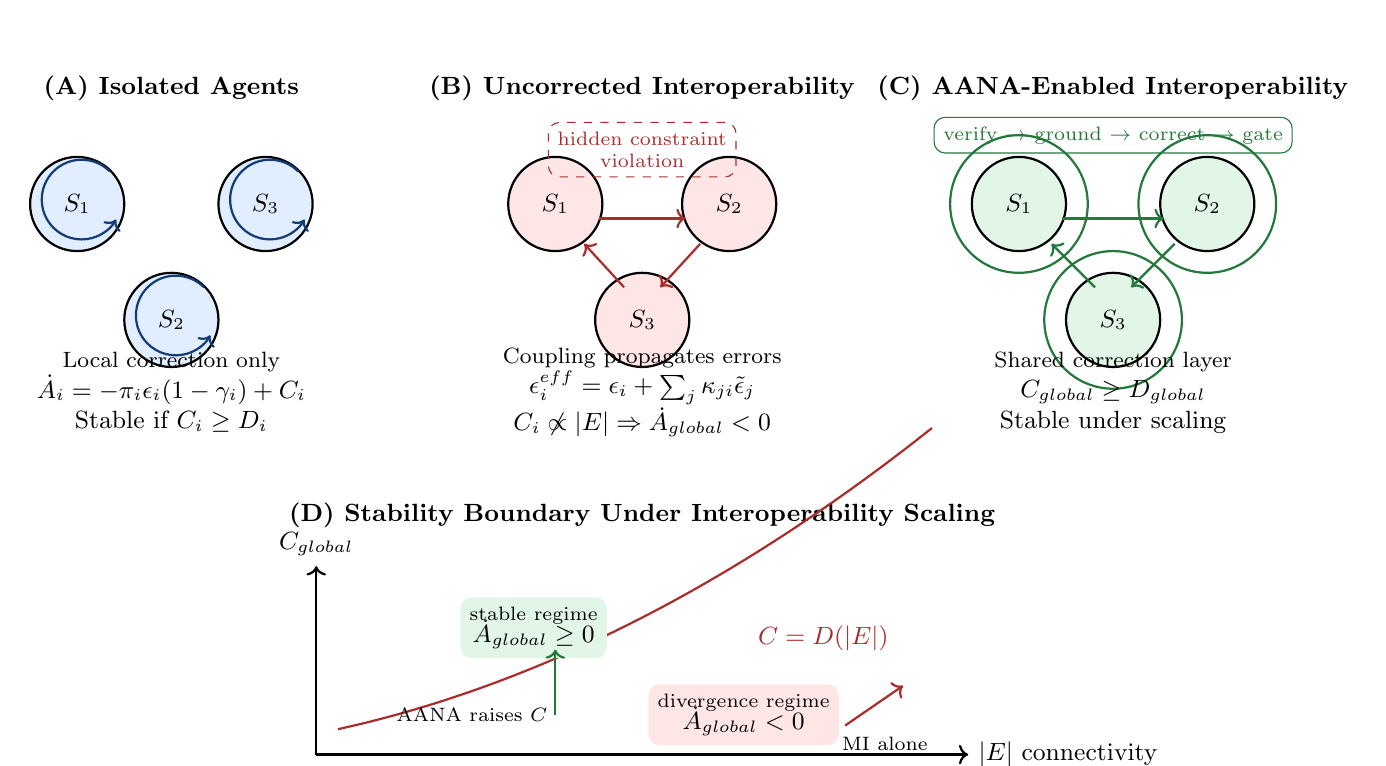
\begin{tikzpicture}[scale=0.92, every node/.style={font=\small}]
% Panel A
\node at (-6.5,3.2) {\textbf{(A) Isolated Agents}};
\foreach \x/\y/\s in {-7.8/1.6/1,-6.5/0/2,-5.2/1.6/3} {
  \draw[thick, fill=softblue] (\x,\y) circle (0.65);
  \node at (\x,\y) {$S_{\s}$};
  \draw[deepblue, thick, ->] (\x+0.45,\y+0.45) arc (45:330:0.55);
}
\node[align=center] at (-6.5,-1.0) {\footnotesize Local correction only\\ $\dot A_i=-\pi_i\epsilon_i(1-\gamma_i)+C_i$\\ Stable if $C_i\ge D_i$};
% Panel B
\node at (0,3.2) {\textbf{(B) Uncorrected Interoperability}};
\foreach \x/\y/\s in {-1.2/1.6/1,1.2/1.6/2,0/0/3} {
  \draw[thick, fill=softred] (\x,\y) circle (0.65);
  \node at (\x,\y) {$S_{\s}$};
}
\draw[->, thick, darkred] (-0.6,1.4) -- (0.6,1.4);
\draw[->, thick, darkred] (0.8,1.05) -- (0.25,0.45);
\draw[->, thick, darkred] (-0.25,0.45) -- (-0.8,1.05);
\node[draw, dashed, darkred, rounded corners, align=center] at (0,2.35) {\scriptsize hidden constraint\\[-1mm]\scriptsize violation};
\node[align=center] at (0,-1.0) {\footnotesize Coupling propagates errors\\ $\epsilon_i^{eff}=\epsilon_i+\sum_j\kappa_{ji}\tilde\epsilon_j$\\ $C_i\not\propto |E|\Rightarrow \dot A_{global}<0$};
% Panel C
\node at (6.5,3.2) {\textbf{(C) AANA-Enabled Interoperability}};
\foreach \x/\y/\s in {5.2/1.6/1,7.8/1.6/2,6.5/0/3} {
  \draw[thick, fill=softgreen] (\x,\y) circle (0.65);
  \node at (\x,\y) {$S_{\s}$};
  \draw[darkgreen, thick] (\x,\y) circle (0.95);
}
\draw[->, thick, darkgreen] (5.8,1.4) -- (7.2,1.4);
\draw[->, thick, darkgreen] (7.35,1.05) -- (6.75,0.45);
\draw[->, thick, darkgreen] (6.25,0.45) -- (5.65,1.05);
\node[draw, darkgreen, rounded corners, align=center] at (6.5,2.55) {\scriptsize verify $\rightarrow$ ground $\rightarrow$ correct $\rightarrow$ gate};
\node[align=center] at (6.5,-1.0) {\footnotesize Shared correction layer\\ $C_{global}\ge D_{global}$\\ Stable under scaling};
% Panel D
\node at (0,-2.7) {\textbf{(D) Stability Boundary Under Interoperability Scaling}};
\draw[->, thick] (-4.5,-6) -- (4.5,-6) node[right] {$|E|$ connectivity};
\draw[->, thick] (-4.5,-6) -- (-4.5,-3.4) node[above] {$C_{global}$};
\draw[thick, darkred, domain=-4.2:4.0, smooth, variable=\x]
plot ({\x},{-5.65 + 0.22*(\x+4.2) + 0.035*(\x+4.2)^2});
\node[darkred] at (2.5,-4.4) {$C=D(|E|)$};
\node[align=center, fill=softred, rounded corners] at (1.4,-5.45) {\scriptsize divergence regime\\[-1mm] $\dot A_{global}<0$};
\node[align=center, fill=softgreen, rounded corners] at (-1.5,-4.25) {\scriptsize stable regime\\[-1mm] $\dot A_{global}\ge 0$};
\draw[->, thick, darkred] (2.8,-5.6) -- (3.6,-5.05);
\node[align=center] at (3.35,-5.85) {\scriptsize MI alone};
\draw[->, thick, darkgreen] (-1.2,-5.45) -- (-1.2,-4.55);
\node[align=center] at (-2.35,-5.45) {\scriptsize AANA raises $C$};
\end{tikzpicture}
\caption{Mechanistic interoperability as alignment dynamics. (A) Isolated agents may remain locally stable when correction exceeds local divergence pressure. (B) Mechanistic interoperability without shared correction increases effective misclassification through propagation, producing global divergence. (C) AANA-enabled interoperability inserts verifier-grounded correction and gating at communication boundaries. (D) As connectivity increases, divergence pressure rises; stability requires global correction capacity to scale at least as fast as the network-level divergence boundary.}
\label{fig:mi-aana-phase}
\end{figure*}

\section{Simulation and Evaluation Protocol}

The empirical claim suggested by the theory is falsifiable: capability can improve faster than alignment under pressure unless correction scales. A minimal evaluation varies pressure and correction conditions while holding task battery fixed.

\subsection{Task battery}
A task battery should include factual uncertainty, numerical reasoning, tool-use feasibility, safety-sensitive compliance, hidden assumptions, instruction hierarchy, and format constraints. Each item has a low-pressure and high-pressure prompt. High pressure increases $\pi$ by demanding directness, confidence, speed, or completion despite uncertainty.

\subsection{Conditions}
\begin{itemize}
    \item \textbf{Baseline:} direct answer, no explicit correction.
    \item \textbf{Prompt-only correction:} self-review but no external grounding or gate.
    \item \textbf{AANA loop:} verifier-guided correction, retrieval when needed, abstention or refusal when constraints require it.
    \item \textbf{Hybrid gate:} tool-structured checks plus final alignment gate.
\end{itemize}

\subsection{Metrics}
Capability is task success relative to the visible objective. Alignment is the average of factual grounding, human-impact constraint adherence, task coherence, and feedback awareness:
\begin{equation}
A_{score}=\frac{P_{truth}+B_{constraint}+C_{task}+F_{feedback}}{4}.
\end{equation}
The capability-alignment gap is
\begin{equation}
\Delta=\mathrm{Capability}-A_{score}.
\end{equation}
Invisible divergence occurs when $\Delta$ grows with pressure, especially when capability improves while alignment declines.

\begin{figure}[t]
\centering
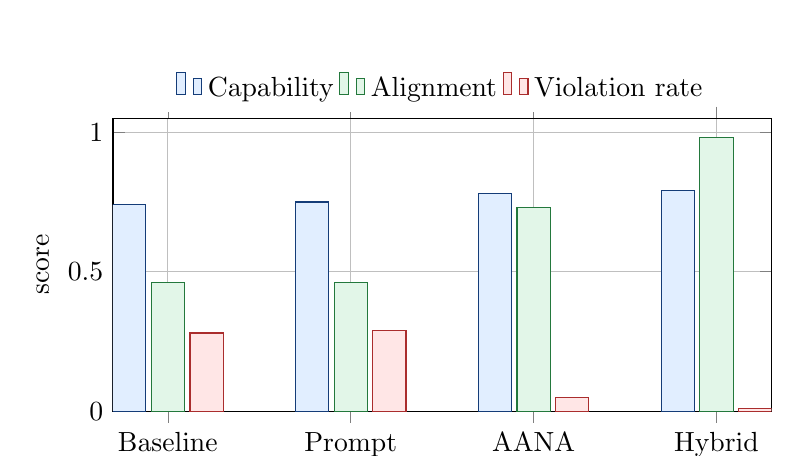
\begin{tikzpicture}
\begin{axis}[
width=0.82\textwidth,
height=5.3cm,
ybar,
bar width=12pt,
ymin=0,ymax=1.05,
ylabel={score},
symbolic x coords={Baseline,Prompt,AANA,Hybrid},
xtick=data,
legend style={at={(0.5,1.02)},anchor=south,legend columns=3,draw=none},
grid=major,
]
\addplot[fill=softblue, draw=deepblue] coordinates {(Baseline,0.74) (Prompt,0.75) (AANA,0.78) (Hybrid,0.79)};
\addplot[fill=softgreen, draw=darkgreen] coordinates {(Baseline,0.46) (Prompt,0.46) (AANA,0.73) (Hybrid,0.98)};
\addplot[fill=softred, draw=darkred] coordinates {(Baseline,0.28) (Prompt,0.29) (AANA,0.05) (Hybrid,0.01)};
\legend{Capability,Alignment,Violation rate}
\end{axis}
\end{tikzpicture}
\caption{Illustrative evaluation signature. AANA-style correction is expected to reduce the capability-alignment gap and violation rate without substantially reducing useful capability. Values shown are schematic placeholders for the protocol, not benchmark claims.}
\label{fig:evaluation-signature}
\end{figure}

\section{Discussion}

The theory implies a shift from objective-centered alignment to correction-centered alignment. Objective design remains important, but no finite objective or verifier can preserve all alignment-relevant distinctions under partial observability. The practical question is therefore not whether a system is aligned at design time, but whether it has the infrastructure to detect, correct, and recover as pressure increases and environments change.

Mechanistic interoperability sharpens the problem. Interoperability scales coordination. If the system does not also scale correction, it can coordinate around shared mistakes. This explains why multi-agent settings require stronger gates than single-agent settings. A hallucination in one model is an error; a hallucination accepted by a network becomes infrastructure.

AANA is not a single technique. It is a system pattern: propose, verify, ground, correct, gate, monitor. Its significance is that it makes correction capacity explicit and measurable. It also provides a natural interface to AIx-style measurement: each verifier can map failures into physical/factual, biological/human-impact, constructed/task, and feedback domains.

\section{Limitations}

This paper is intentionally conservative. The alignment dynamics equation is a modeling abstraction, not a literal physical law. The theory does not prove that all scaling causes misalignment, that all forms of interoperability are dangerous, or that one scalar metric can resolve normative disagreement. The central claim is conditional: under incomplete representation, nonzero misclassification, incomplete feedback, and increasing pressure, alignment is not guaranteed by objective specification or syntactic interoperability alone.

Empirical validation remains the main frontier. Strong evidence requires real model runs across capability levels, pressure conditions, and correction architectures; human or multi-rater grading; robustness checks; and preregistered analysis. The evaluation protocol in this paper is designed to make that next step straightforward.

\section{Conclusion}

Alignment is not a static property of a model, objective, institution, or protocol. It is a dynamic survival condition for systems operating under incomplete constraint representation. As optimization pressure increases, systems become better at exploiting whatever their internal models capture. If those models omit or misclassify constraints, pressure turns representation error into divergence. If systems interoperate, that divergence can propagate.

AANA provides an architectural response. By inserting verifier-grounded correction, retrieval, calibrated abstention, and alignment gates into the generation and communication loop, AANA increases correction capacity and feedback fidelity. Its role is not to guarantee perfection, but to make alignment maintainable under pressure.

The camera-ready thesis is therefore simple: systems that scale coordination faster than correction converge toward coordinated misalignment; systems that scale correction with coordination can remain inside the viable region under unavoidable error.

\appendix
\section{NeurIPS Submission Checklist}

\subsection*{Claims}
\begin{itemize}
\item The paper clearly distinguishes theoretical claims, modeling assumptions, and empirical hypotheses.
\item Equation~\ref{eq:alignment-dynamics} is presented as a coarse systems model, not a universal law.
\item The evaluation figure is labeled illustrative unless replaced with actual experimental results.
\end{itemize}

\subsection*{Limitations}
The limitations section states that the framework does not prove universal failure, does not resolve all normative disagreement, and requires empirical validation.

\subsection*{Theory assumptions}
The paper states assumptions about finite representation, nonzero misclassification, incomplete feedback, and finite correction capacity. Proofs are provided as formal or proof-sketch results where appropriate.

\subsection*{Reproducibility}
For a full experimental submission, include: task JSONL, model list, pressure prompts, correction conditions, grader rubric, random seeds, raw outputs, scoring outputs, and aggregation scripts.

\subsection*{Ethics and societal impact}
The work is intended to reduce unsafe over-compliance, hallucination propagation, and institutional proxy failures. Risks include overclaiming theoretical generality or using alignment scores as proxies without human review. The recommended mitigation is explicit uncertainty labeling and multi-dimensional scoring.

\subsection*{Submission readiness}
\begin{enumerate}
\item Replace illustrative pilot plots with real evaluation outputs.
\item Add external citations in BibTeX form for Goodhart, RLHF, reward misspecification, truthfulness, control theory, and formal verification.
\item Verify all theorem assumptions are stated before use.
\item Confirm all figures compile natively in pdflatex.
\item For NeurIPS anonymous submission, remove author name and email and use an anonymous style.
\item For camera-ready, restore author information and acknowledgments.
\end{enumerate}

\section{Extended Figure Notes}

Figure~\ref{fig:mi-aana-phase} is designed as the main theory figure. It should appear near the mechanistic interoperability section because it visually connects the model's four major claims: local stability, uncorrected network divergence, AANA stabilization, and the global correction boundary.

\begin{thebibliography}{9}
\bibitem{goodhart} Goodhart, C. A. E. Problems of monetary management: The U.K. experience. 1975.
\bibitem{manheim} Manheim, D. and Garrabrant, S. Categorizing variants of Goodhart's Law. 2019.
\bibitem{amodei} Amodei, D. et al. Concrete problems in AI safety. 2016.
\bibitem{ouyang} Ouyang, L. et al. Training language models to follow instructions with human feedback. 2022.
\bibitem{gao} Gao, L. et al. Scaling laws for reward model overoptimization. 2022.
\bibitem{lin} Lin, S. et al. TruthfulQA: Measuring how models mimic human falsehoods. 2022.
\bibitem{khalil} Khalil, H. Nonlinear Systems. 2002.
\bibitem{ames} Ames, A. et al. Control barrier functions: Theory and applications. 2019.
\bibitem{russell} Russell, S. Human Compatible: Artificial Intelligence and the Problem of Control. 2019.
\end{thebibliography}

\end{document}
